\documentclass{article}
\usepackage[a4paper, margin=0.75in]{geometry}
\usepackage{amsmath}
\usepackage{amsthm}
\usepackage{amsfonts}
\usepackage{graphicx}
\allowdisplaybreaks
\author{Mostafa Hassanein}
\title{
  MTH-645 Optimization Techniques \\
  Assignment (2)}
\date{05 March 2026}
\begin{document}

\maketitle

\newpage

\section*{1}

 Carry out three steps of the conjugate gradient method to find the minimum point of the functions:

 \begin{align*}
  (i) F(x)  &= 4x_1^2 + x_1 x_2 + 2x_2^2 - 19 x_1 - 14 x_2 &&\\
  (ii) F(x) &= x_1^2 x_2^2 + (x_1 - 3)^2 + (x_2 - 2)^2.
 \end{align*}

Start at $x = (0, 0)$ and use calculus to find the minimum in each conjugate direction.

Comment on your result after the three steps in comparison with the actual minimum point.

\begin{center}
  \textbf{\underline{Solution:}}  
\end{center}

We'll use the Fletcher-Reeves algorithm, which is given by:
\begin{figure}[h]
    \centering
    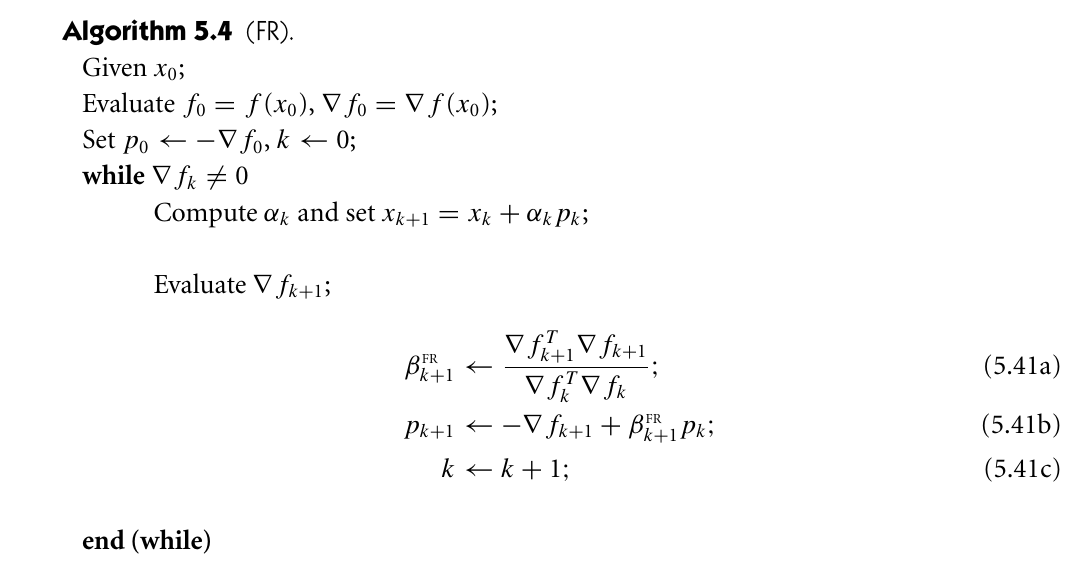
\includegraphics{./fletcher-reeves-method.png}
\end{figure}

\subsection*{i. \underline{$F(x)  = 4x_1^2 + x_1 x_2 + 2x_2^2 - 19 x_1 - 14 x_2$}}

\begin{align*}
  F_{x_1} &= 8x_1 + x_2 - 19 &&\\ 
  F_{x_2} &= x_1 + 4 x_2 - 14 &&\\
  \nabla F &= (8x_1 + x_2 - 19, \: x_1 + 4 x_2 - 14).
\end{align*}

\noindent
\underline{iteration 1:}
\begin{align*}
  x_0 &= (0, 0) &&\\
  &&\\
  f_0 &= 0 &&\\
  &&\\
  \nabla f_0 &= (-19, -14) &&\\
  &&\\
  p_0 &= -\nabla(f_0) = (19, 14) &&\\
  &&\\
  F(\alpha_0) 
  &= 4(19 \alpha_0)^2  + (19 \alpha_0)(14 \alpha_0) + 2(14 \alpha_0)^2 - 19(19 \alpha_0) - 14(14 \alpha_0) &&\\
  &= 1444 \alpha_0^2 + 266 \alpha_0^2 + 392 \alpha_0^2 - 361 \alpha_0 - 196 \alpha_0 &&\\
  &= 2102 \alpha_0^2 -557 \alpha_0 &&\\
  &&\\
  F(\alpha)^\prime &= 4204 \alpha_0 - 557 = 0 &&\\
  &\implies \alpha_0 = 0.13 &&\\
  &&\\
  x_{1} &= x_0 + \alpha_0 p_0 &&\\
  &= (0, 0) + 0.13 (19, 14) = (2.47, 1.82) &&\\
  &&\\
  f_1 &= -36.9 &&\\
  &&\\
  \nabla f_1 &=  (2.58, -4.25) &&\\
  &&\\
  \beta_{1} &= \frac{\nabla f_1^T \nabla f_1}{\nabla f_0^T \nabla f_0} &&\\
  &= 0.04 &&\\
  &&\\
  p_1 &= -\nabla f_1 + \beta_1 p_0 &&\\
  &= (-2.58, 4.25) + 0.04 (19, 14) = (-1.82, 4.81).
\end{align*}
\newline

\noindent
\underline{iteration 2:}
\begin{align*}
  F(\alpha_1) 
  &= 4(2.47 - 1.82 \alpha_1)^2  + (2.47 - 1.82 \alpha_1)(1.82 + 4.81 \alpha_1) + 2(1.82 + 4.81 \alpha_1)^2 - 19(2.47 - 1.82 \alpha_1) - 14(1.82 + 4.81 \alpha_1) &&\\
  &= 50.7676 \alpha_1^2 - 25.14 \alpha_1 - 36.9 &&\\
  &&\\
  F(\alpha_1)^\prime &= 101.54 \alpha_1 - 25.14 = 0 &&\\
  &\implies \alpha_1 = 0.25 &&\\
  &&\\
  x_2 &= x_1 + \alpha_1 p_1 &&\\
  &= (2.47, 1.82) + 0.25 (-1.82, 4.81) = (2.02, 3.02) &&\\
  &&\\
  f_2 &= -40 &&\\
  &&\\
  \nabla f_2 &=  (0.18, 0.1) &&\\
  &&\\
  \beta_{2} &= \frac{\nabla f_2^T \nabla f_2}{\nabla f_1^T \nabla f_1} &&\\
  &= 0.0017 &&\\
  &&\\
  p_2 &= -\nabla f_2 + \beta_2 p_1 &&\\
  &= (-0.18, -0.1) + 0.0017 (-1.82, 4.81) = (-0.18, -0.092).
\end{align*}
\newline

\noindent
\underline{iteration 3:}
\begin{align*}
  F(\alpha_2) 
  &= 4(2.02 - 0.18 \alpha_2)^2  + (2.02 - 0.18 \alpha_2)(3.02 -0.092 \alpha_2) + 2(3.02 -0.092 \alpha_2)^2 - 19(2.02 - 0.18 \alpha_2) - 14(3.02 -0.092 \alpha_2) &&\\
  &= 0.16 \alpha_2^2 - 0.04 \alpha_2 - 40 &&\\
  &&\\
  F(\alpha_2)^\prime &= 0.32 \alpha_2 -0.04 = 0 &&\\
  &\implies \alpha_2 = 0.125 &&\\
  &&\\
  x_3 &= x_2 + \alpha_2 p_2 &&\\
  &= (2.02, 3.02) + 0.125 (-0.18, -0.092) = (2, 3) &&\\
  &&\\
  f_3 &= -40.
\end{align*}

\noindent
\textbf{\underline{Comments:}} 

Since $F(x)$ is a quadratic function , then we expect exact convergence in $n = 2$ iterations (where n is the dimensionality).

The actual minimum $F^*(x)= -40$ occurs at $x^* = (2, 3)$.

Our solution did indeed converge to $x^*$ (if not for the round-off errors) in the second iteration. The third iteration removed the round-off errors, and achieved exact convergence.
\newline
\newline

\subsection*{ii. \underline{$F(x) = x_1^2 x_2^2 + (x_1 - 3)^2 + (x_2 - 2)^2$}}

\begin{align*}
  F_{x_1} &= 2x_1 x_2^2 + 2(x_1 - 3) &&\\ 
  F_{x_2} &= 2x_1^2 x_2 + 2(x_2 - 2) &&\\
  \nabla F &= (2x_1 x_2^2 + 2(x_1 - 3), \: 2x_1^2 x_2 + 2(x_2 - 2)).
\end{align*}

\noindent
\underline{iteration 1:}
\begin{align*}
  x_0 &= (0, 0) &&\\
  % &&\\
  f_0 &= 13 &&\\
  &&\\
  \nabla f_0 &= (-6, -4) &&\\
  &&\\
  p_0 &= -\nabla(f_0) = (6, 4) &&\\
  &&\\
  F(\alpha_0) 
  &= (6\alpha_0)^2(4\alpha_0)^2 + (6\alpha_0 -3)^2 + (4\alpha_0 -2)^2 &&\\
  &= 576 \alpha_0^4 + 52 \alpha_0^2 - 52\alpha_0 + 13 &&\\
  &&\\
  F(\alpha)^\prime &= 2304 \alpha_0^3 + 104 \alpha_0 - 52 = 0 &&\\
  &\implies \alpha_0 = 0.23 \qquad \text{(This is the only real solution, the remaining 2 solutions are complex.)} &&\\
  &&\\
  x_{1} &= x_0 + \alpha_0 p_0 &&\\
  &= (0, 0) + 0.23 (6, 4) = (1.38, 0.92) &&\\
  &&\\
  f_1 &= 5.40 &&\\
  &&\\
  \nabla f_1 &=  (-0.90, 1.34) &&\\
  &&\\
  \beta_{1} &= \frac{\nabla f_1^T \nabla f_1}{\nabla f_0^T \nabla f_0} &&\\
  &= 0.05 &&\\
  &&\\
  p_1 &= -\nabla f_1 + \beta_1 p_0 &&\\
  &= (0.90, -1.34) + 0.05 (6, 4) = (1.2, -1.14).
\end{align*}
\newline

\noindent
\underline{iteration 2:}
\begin{align*}
  F(\alpha_1) 
  &= (1.38+ 1.2\alpha_1)^2 (0.92 - 1.14 \alpha_1)^2 + (1.38+ 1.2\alpha_1 - 3)^2 + (0.92 - 1.14 \alpha_1 - 2)^2 &&\\
  &= 1.87 \alpha_1^4 + 1.28 \alpha^3 - 0.51 \alpha_1^2 - 2.62 \alpha_1 + 5.40 &&\\
  &&\\
  F(\alpha_1)^\prime &= 7.48 \alpha_1^3 +3.84 \alpha_1^2 - 1.02 \alpha_1 - 2.62 = 0 &&\\
  &\implies \alpha_1 = 0.62 &&\\
  &&\\
  x_2 &= x_1 + \alpha_1 p_1 &&\\
  &= (1.38, 0.92) + 0.62 (1.2, -1.14) = (2.12, 0.21) &&\\
  &&\\
  f_2 &= 4.18 &&\\
  &&\\
  \nabla f_2 &=  (-1.57, -1.69) &&\\
  &&\\
  \beta_{2} &= \frac{\nabla f_2^T \nabla f_2}{\nabla f_1^T \nabla f_1} &&\\
  &= 2.04 &&\\
  &&\\
  p_2 &= -\nabla f_2 + \beta_2 p_1 &&\\
  &= (1.57, 1.69) + 2.04 (1.2, -1.14) = (4.02, -0.64).
\end{align*}
\newline

\noindent
\underline{iteration 3:}
\begin{align*}
  F(\alpha_2) 
  &= (2.12 + 4.02 \alpha_2)^2 (0.21 - 0.64 \alpha_2)^2
  + (2.12 + 4.02 \alpha_2 - 3)^2
  + (0.21 - 0.64 \alpha_2 - 2)^2 &&\\
  &= 6.62 \alpha_2^4 + 2.64 \alpha_2^3 + 14.54 \alpha_2^2 - 5.24 \alpha_2 + 4.18 &&\\
  &&\\
  F(\alpha_2)^\prime &= 26.48 \alpha_2^3 + 7.92 \alpha_2^2 + 29.08 \alpha_2 - 5.24 = 0 &&\\
  &\implies \alpha_2 = 0.17 &&\\
  &&\\
  x_3 &= x_2 + \alpha_2 p_2 &&\\
  &= (2.12, 0.21) + 0.17 (4.02, -0.64) = (2.80, 0.10) &&\\
  &&\\
  f_3 &= 3.73.
\end{align*}

\noindent
\textbf{\underline{Comments:}} 

Since $F(x)$ is a quartic function (and, thus not a quadratic), then we don't expect convergence in n iterations (where n is the dimensionality).

The actual minimum $F^*(x)= 3.58$ occurs at $x^* = (2.86, 0.22)$.

The distance from $x_3$ to $x^*$ (in the Euclidean 2-norm) is: $||x_3 - x^*||_2 = 0.134 = 13.4\%$.

This is a large error. 

Conclusion: More iterations are required for convergence.
\newpage

\section*{2.}
(i). Certify that the following Davidon-Fletcher-Powell (DFP) updating-formula satisfies the condition for a Quasi-Newton method.

\begin{align*}
  A_{k+1} = A_k 
  - \frac{A_k y_k y_k^T A_k}{y_k^T A_k y_k}  
  + \frac{s_k s_k^T}{s_k^T y_k}
\end{align*}

where,
\begin{align*}
  A_k \approx H^{-1}, \qquad s_k = x_{k+1} - x_k, \qquad y_k = g_{k+1} - g_k
\end{align*}

(ii). Hence, carry out two steps to minimize $F(x)$ of problem (1)(i) using calculus to find the minimum in each search direction.
\newline

(iii). Compare with the updating formula given by:
\begin{align*}
  B_{k+1} = B_k + \frac{z z^T}{z^T s_k}
\end{align*}
where,
\begin{align*}
  z = y_k - B_k s_k, \qquad B_k \approx H.
\end{align*}

\begin{center}
  \textbf{\underline{Solution:}}  
\end{center}

\subsection*{i. Show that $A_{k+1}$ satisfies the Quasi-Newton Secant Equation: $A_{k+1} y_k = s_k$}

\begin{proof}
  \begin{align*}
    A_{k+1} 
    = A_k 
    - \frac{A_k y_k y_k^T A_k}{y_k^T A_k y_k}  
    + \frac{s_k s_k^T}{s_k^T y_k}
  \end{align*}

  multiply by $y_k$ on the right:

  \begin{align*}
    A_{k+1} y_k 
    = A_k y_k
    - \frac{A_k y_k y_k^T A_k y_k}{y_k^T A_k y_k}  
    + \frac{s_k s_k^T y_k}{s_k^T y_k}
  \end{align*}

  Group:

  \begin{align*}
    A_{k+1} y_k 
    = A_k y_k
    - \frac{A_k y_k \left(y_k^T A_k y_k\right)}{\left(y_k^T A_k y_k\right)}  
    + \frac{s_k \left(s_k^T y_k\right)}{\left(s_k^T y_k\right)}
  \end{align*}

  Simplify:
  \begin{align*}
    A_{k+1} y_k 
    = A_k y_k
    - A_k y_k
    + s_k 
    = s_k.
  \end{align*}
\end{proof}

\newpage
\subsection*{ii. Minimize: $F(x) = 4x_1^2 + x_1 x_2 + 2x_2^2 - 19 x_1 - 14 x_2$}

We'll use the BFGS algorithm, which is given by:
\begin{figure}[h]
    \centering
    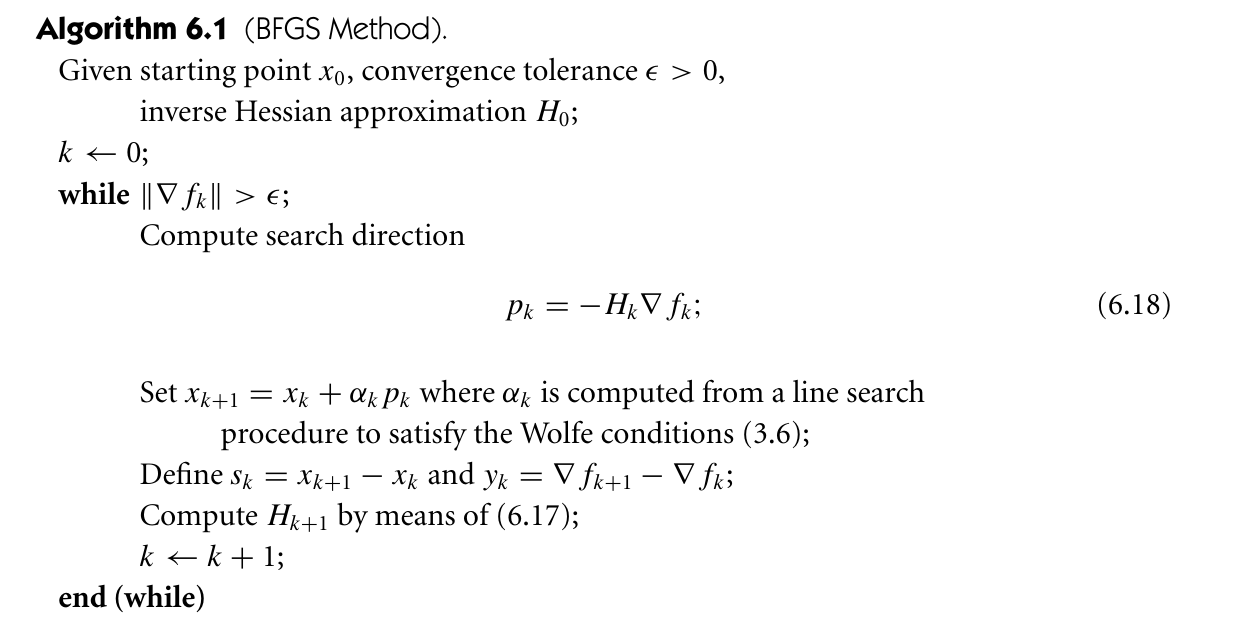
\includegraphics{./BFGS-method.png}
\end{figure}

\begin{align*}
  F_{x_1} &= 8x_1 + x_2 - 19 &&\\ 
  F_{x_2} &= x_1 + 4 x_2 - 14 &&\\
  \nabla F &= (8x_1 + x_2 - 19, \: x_1 + 4 x_2 - 14).
\end{align*}

\noindent
\underline{iteration 1:}
\begin{align*}
  x_0 &= (0, 0) &&\\
  &&\\
  f_0 &= 0 &&\\
  &&\\
  A_0 &= I &&\\
  &&\\
  \nabla f_0 &= (-19, -14) &&\\
  &&\\
  p_0 &= -A_0 \nabla f_0 &&\\
  &= -I (-19, -14) = (19, 14) &&\\
  &&\\
  F(\alpha_0) 
  &= 4(19 \alpha_0)^2  + (19 \alpha_0)(14 \alpha_0) + 2(14 \alpha_0)^2 - 19(19 \alpha_0) - 14(14 \alpha_0) &&\\
  &= 1444 \alpha_0^2 + 266 \alpha_0^2 + 392 \alpha_0^2 - 361 \alpha_0 - 196 \alpha_0 &&\\
  &= 2102 \alpha_0^2 -557 \alpha_0 &&\\
  &&\\
  F(\alpha)^\prime &= 4204 \alpha_0 - 557 = 0 &&\\
  &\implies \alpha_0 = 0.13 &&\\
  &&\\
  x_{1} &= x_0 + \alpha_0 p_0 &&\\
  &= (0, 0) + 0.13 (19, 14) = (2.47, 1.82) &&\\
  &&\\
  f_1 &= -36.9 &&\\
  &&\\
  \nabla f_1 &=  (2.58, -4.25) &&\\
  &&\\
  s_0 &= x_1 - x_0 = (2.47, 1.82) &&\\
  &&\\
  y_0 &= g_1 - g_0 = (21.58, 9.75) &&\\
  &&\\
  A_1
  &= A_0
  - \frac{A_0 y_0 y_0^T A_0}{y_0^T A_0 y_0}  
  + \frac{s_0 s_0^T}{s_0^T y_0} &&\\
  &= I
  - \frac{I \begin{bmatrix} 21.58 \\ 9.75 \\ \end{bmatrix} \begin{bmatrix} 21.58 & 9.75 \\ \end{bmatrix} I}{\begin{bmatrix} 21.58 & 9.75 \\ \end{bmatrix} I \begin{bmatrix} 21.58 \\ 9.75 \\ \end{bmatrix}}  
  + \frac{\begin{bmatrix} 2.47 \\ 1.82 \\ \end{bmatrix} \begin{bmatrix} 2.47 & 1.82 \\ \end{bmatrix}}{\begin{bmatrix} 2.47 & 1.82 \\ \end{bmatrix} \begin{bmatrix} 21.58 \\ 9.75 \\ \end{bmatrix}} &&\\
  &= I
  - \frac{\begin{bmatrix} 
    465.70 & 210.41 \\
    210.41 & 95.10 \\
    \end{bmatrix}}{560.76}  
  + \frac{\begin{bmatrix} 
    6.10 & 4.50 \\
    4.50 & 3.31 \\
    \end{bmatrix}}{71.1} &&\\
    &= I
  - \begin{bmatrix} 
    0.83 & 0.38 \\
    0.38 & 0.17 \\
    \end{bmatrix}
  + \begin{bmatrix} 
    0.09 & 0.06 \\
    0.06 & 0.05 \\
    \end{bmatrix} &&\\
  &= \begin{bmatrix} 
    0.26 & -0.32 \\
    -0.32 & 0.88 \\
    \end{bmatrix} &&\\
  &&\\
  p_1 &= -A_1 \nabla f_1 &&\\
  &= \begin{bmatrix} 
    -0.26 & 0.32 \\
    0.32 & -0.88 \\
    \end{bmatrix} 
    \begin{bmatrix} 
    2.58 \\
    -4.25 \\
    \end{bmatrix}
  &&\\
  &= \begin{bmatrix} 
    -2.03 \\
    4.57 \\
    \end{bmatrix}
  &&\\
\end{align*}
\newline

\noindent
\underline{iteration 2:}
\begin{align*}
  F(\alpha_1) 
  &= 4(2.47 - 2.03 \alpha_1)^2  + (2.47 - 2.03 \alpha_1)(1.82 + 4.57 \alpha_1) + 2(1.82 + 4.57 \alpha_1)^2 - 19(2.47 - 2.03 \alpha_1) - 14(1.82 + 4.57 \alpha_1) &&\\
  &= 48.98 \alpha_1^2 - 24.66 \alpha_1 - 36.89 &&\\
  &&\\
  F(\alpha_1)^\prime &= 97.96 \alpha_1 - 24.66 = 0 &&\\
  &\implies \alpha_1 = 0.25 &&\\
  &&\\
  x_{1} &= x_1 + \alpha_1 p_1 &&\\
  &= (2.47, 1.82) + 0.25 (-2.03, 4.57) = (1.96, 2.96) &&\\
  &&\\
  f_1 &= -39.99.
\end{align*}
\newline

\subsection*{iii. Compare the Update Formulas $A_{k+1}$ and $B_{k+1}$:}



\end{document}